\section{Квантовая яма CdTe--HgTe--CdTe\\ в модели сильной связи}
В этом разделе будет построена модель сильной связи, эквивалентная $k\cdot p$ гамильтониану
\eqref{kane_ham}. Численно диагонализуя её, можно независимо получить уровни размерного 
квантования.
\subsection{Модель однородного полупроводника}
Модель представляет из себя 
кубическую решётку из атомов, на каждом из которых ``сидят'' состояния
с $p_x$, $p_y$, $p_z$ и $s$--орбиталями и двумя 
возможными проекцими спина.

Для написания
спин--орбитального гамильтониана $p$--зоны необходимо перейти к состояниям с определённым
полным моментом. Эти состояния выражаются через $p_x$, $p_y$, $p_z$ орбитали через
коэффициенты Клебша--Гордана.

Спин--орбитальное взаимодействие приводит к расщеплению состояний с моментами $\frac32$ и
$\frac12$.
Состояниями с полным моментом $\frac{1}{2}$ 
можно пренебречь, если спин--орбитальное взаимодейтвие велико. Таким образом, в каждом
узле решётки остаётся пара $s$--орбиталей, формирующая валентную зону, и четыре состояния
с полным моментом $\frac{3}{2}$. Матричные элементы перекрытия между состояниями на соседних
узлах выражаются через перекрытия $s$ и $p$ орбиталей с использованием их выражений через
коэффициенты Клебша--Гордана.

Определим матричные элементы $t_\parallel$ и $t_\perp$ для перекрытия соседних $p$--орбиталей,
расположенных соответственно <<вдоль>> и <<поперёк>>, $\frac{-iP}{2}$ для перекрытия
$s$ и $p$--орбитали и $-\frac{1}{2m_s}$ --- для $s$--орбиталей. Через них полный гамильтониан
сильной связи записывается в импульсном представлении в виде огромной матрицы $6\times6$. 

\begin{equation}
    \label{hfull}
    H_{\mathrm{full}} = \begin{pmatrix}
                            H_c & T \\
                            T^\dagger & H_v
                        \end{pmatrix},
\end{equation}
Матрицы $H_c$, $T$, $H_v$ определены формулами \eqref{H_conduction}--\eqref{H_valence}, см.
стр.~\pageref{H_conduction}.
Этот гамильтониан можноразложить по малым $p$,
в результате чего получится гамильтониан Латтинжера:
\begin{multline}
    H_v = \frac{\hbar^2}{2ma^2}\left\{-\left(\gamma_1 + \frac{5}{2}\gamma_2\right) k^2 + 
        2\gamma_2(k_x^2J_x^2 + k_y^2J_y^2 + k_z^2J_z^2) + \right. \\
        \left.\vphantom{\left(\frac{1}{2}\right)} 
            +4\gamma_3(k_x k_y J_x J_y + k_x k_z J_x J_z + k_y k_z J_y J_z) \right\}
\end{multline}
Здесь $J_i$ --- операторы момента для спина $\frac{3}{2}$, $a$ --- постоянная решётки,
$m$ --- масса электрона,
\begin{equation}
    \begin{gathered}
        \frac{\hbar^2}{2ma^2}\gamma_1 = \frac13 t_\parallel\\
        \frac{\hbar^2}{2ma^2}\gamma_2 = \frac16(t_\parallel - t_\perp)\\
        \gamma_3 = 0\\
    \end{gathered}
\end{equation}
Разложение $H_c$ и $T$ тривиально.
Всё это вместе воспроизводит модель Кейна, которую обычно получают в $k \cdot p$ приближении.

Коэффициенты перескока в сильной связи можно зафиксировать требованием, чтобы при малых $p$ 
воспроизводился $k\cdot p$ гамильтониан с значениями параметров, известных из эксперимента
\cite{Novik2005}. 

%\section{Коэффициенты Клебша--Гордана}
%\label{app:tb}
%Состояния с определённым полным моментом выражаются через $p_x$, $p_y$, $p_z$ орбитали через
%коэффициенты Клебша--Гордана:
%\begin{equation}
%	\label{transform1}
%	\begin{gathered}
%        \Psi_{\frac{3}{2},\frac{3}{2}} = \frac{X + iY}{\sqrt{2}}\alpha\\
%        \Psi_{\frac{3}{2}, \frac{1}{2}} = \sqrt{\frac{1}{3}}\frac{X + iY}{\sqrt{2}}\beta -
%                                         \sqrt{\frac{2}{3}} Z\alpha\\
%        \Psi_{\frac{3}{2}, -\frac{1}{2}} = -\sqrt{\frac{1}{3}}\frac{X - iY}{\sqrt{2}}\alpha -
%                                         \sqrt{\frac{2}{3}} Z\beta\\
%        \Psi_{\frac{3}{2},-\frac{3}{2}} = -\frac{X - iY}{\sqrt{2}}\beta
%	\end{gathered}
%\end{equation}
%\begin{equation}
%	\label{transform2}
%	\begin{gathered}
%        \Psi_{\frac{1}{2}, \frac{1}{2}} = \sqrt{\frac{2}{3}}\frac{X + iY}{\sqrt{2}}\beta +
%                                         \sqrt{\frac{1}{3}} Z\alpha\\
%        \Psi_{\frac{1}{2}, -\frac{1}{2}} = -\sqrt{\frac{2}{3}}\frac{X - iY}{\sqrt{2}}\alpha-
%                                         \sqrt{\frac{1}{3}} Z\beta\\
%	\end{gathered}
%\end{equation}
%
%Здесь $X,Y,Z$ --- атомные орбитали, $\alpha,\beta$ --- состояния со спином вверх и вниз.

\afterpage{%
    \clearpage% Flush earlier floats (otherwise order might not be correct)
%    \thispagestyle{empty}% empty page style (?)
    \begin{landscape}% Landscape page
        \centering % Center table
        \vspace*{\fill}
        \begin{equation}
            \label{H_conduction}
            H_c = (E_s + \frac{1}{m_s}(3 - \cos{p_x} - \cos{p_y} - \cos{p_z}))I_{2\times2}
        \end{equation}
        \begin{equation}
            \label{T_matrix}
            T = P\begin{pmatrix}
                    -\frac{1}{\sqrt{2}}(\sin{p_x} + i\sin{p_y}) & \sqrt{\frac{2}{3}}\sin{p_z} &
                     \frac{1}{\sqrt{6}}(\sin{p_x} - i\sin{p_y}) & 0 \\  
                    0 & -\frac{1}{\sqrt{6}}(\sin{p_x} + i\sin{p_y}) & 
                    \sqrt{\frac{2}{3}}\sin{p_z} & \frac{1}{\sqrt{2}}(\sin{p_x} - i\sin{p_y}),
                 \end{pmatrix},
        \end{equation}
        \begin{equation}
            \label{H_valence}
            H_v = 
            \begin{pmatrix}
                (t_\parallel + t_\perp)(\cos{p_x} + \cos{p_y}) + 2t_\perp \cos{p_z} & 0 &
                -\frac{1}{\sqrt{3}}(t_\parallel - t_\perp)(\cos{p_x} - \cos_{p_y}) & 0 \\
                0 & \left(\frac{t_\parallel}{3} + \frac{5t_\perp}{3}\right)(\cos{p_x}+\cos{p_y})+ 
                              \left(\frac{2t_\perp}{3} + \frac{4t_\parallel}{3}\right)\cos{p_z} &
                0 & -\frac{1}{\sqrt{3}}(t_\parallel - t_\perp)(\cos{p_x} - \cos_{p_y})\\
                -\frac{1}{\sqrt{3}}(t_\parallel - t_\perp)(\cos{p_x} - \cos_{p_y}) & 0 &
               \left(\frac{t_\parallel}{3} + \frac{5t_\perp}{3}\right)(\cos{p_x} + \cos{p_y}) + 
                       \left(\frac{2t_\perp}{3} + \frac{4t_\parallel}{3}\right)\cos{p_z} & 0 \\
                0 & -\frac{1}{\sqrt{3}}(t_\parallel - t_\perp)(\cos{p_x} - \cos_{p_y}) &
                0 & (t_\parallel + t_\perp)(\cos{p_x} + \cos{p_y}) + 2t_\perp \cos{p_z}
            \end{pmatrix}
        \end{equation}
    \vspace*{\fill}
    \end{landscape}
    \clearpage% Flush page
}

\subsection{Модель квантовой ямы}
Квантовая яма представляет из себя последовательно расположенные слои CdTe, HgTe и CdTe.
Это можно непосредственно реализовать как модель сильной связи с двумя типами узлов, которую
затем несложно диагонализовать численно. Спектр этой модели состоит из густо расположенных
двумерных зон, соответствующих объёмным состояниям CdTe, и двумерных зон размерного квантования
HgTe, расположенных в запрещённой зоне CdTe.

Для двух уровней размерного квантования можно написать эффективный гамильтониан,
учитывающий только их. Оказывается, что этот гамильтониан при малых $k_x,k_y$ превращается
в две копии 
\eqref{BHZ}, переходящие друг в друга при обращении времени. $\xi$ из гамильтониана \eqref{BHZ} --- это расстояние между уровнями размерного
квантования при $k_x, k_y$. Таким образом, в тот момент, когда два уровня размерного 
квантования пересекаются, эффективный гамильтониан для этих уровней становится 
гамильтонианом топологического изолятора. Согласно \cite{Bernevig2006}, это происходит
при толщине ямы, равной $6.4$ nm. У меня получилось, что критическая толщина равна
$\approx 7.5$ nm.

\begin{figure}[h]
    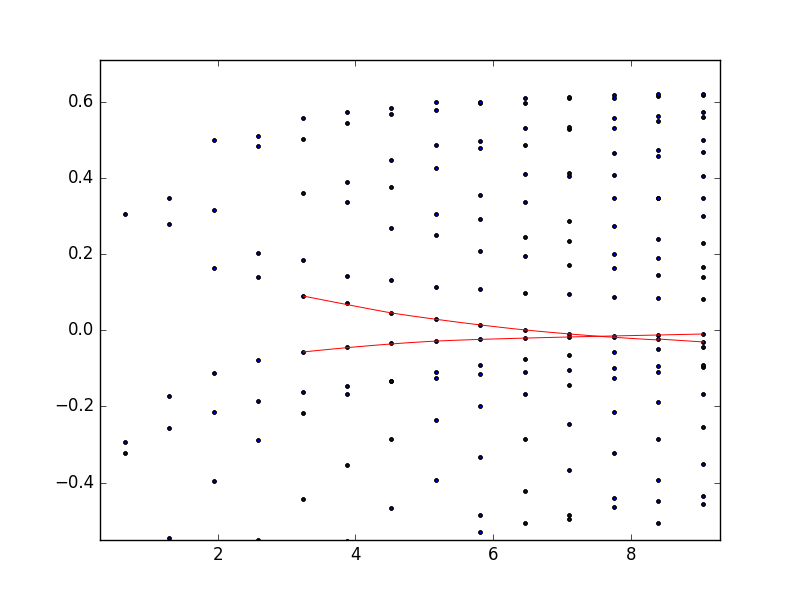
\includegraphics[width=0.8\linewidth]{dim_quant_levels_mod.png}
    \caption{
            На графике изображены уровни размерного квантования, полученные 
            численной диагонализацией, для $k_x, k_y = 0$
            в зависимости от толщины слоя HgTe, nm. Видно, что два уровня размерного
            пересекаютcя при $d \approx 7.5$.
            }
\end{figure}
